\part{Rotating field theory}
\title[Rotating field theory]{Rotating field theory}  
\date{}  
\frame{\titlepage} 

%%%%%%%%%%%%%%%%%%%%%%%%%%%%%%%%%%%%%%%%%%%%%%%%%%%%%%%%%%%%%
%% Conceptual idea of a rotating magnetic field %%
%%%%%%%%%%%%%%%%%%%%%%%%%%%%%%%%%%%%%%%%%%%%%%%%%%%%%%%%%%%%%
\begin{frame}
	\frametitle{Conceptual idea of a rotating magnetic field}
    \begin{figure}
        \centering
        \movie{\includegraphics[height=0.7\textheight]{fig/lec05/Three_phase_coils_rotating_field_preview.png}}{fig/lec05/Three_phase_coils_rotating_field.gif}
        \caption{Animation of a rotating magnetic field produced by three-phase currents in three coils both physically and electrically displaced by $120^\circ$ (inspired by \href{https://perso.univ-lyon1.fr/charles.joubert/web_anim/simen_rotfield_create.html}{C.~Joubert})}
        \label{fig:Three_phase_coils_rotating_field_animation}
    \end{figure}
\end{frame}

%%%%%%%%%%%%%%%%%%%%%%%%%%%%%%%%%%%%%%%%%%%%%%%%%%%%%%%%%%%%%
%% MMF distribution of a single-phase coil %%
%%%%%%%%%%%%%%%%%%%%%%%%%%%%%%%%%%%%%%%%%%%%%%%%%%%%%%%%%%%%%
\begin{frame}
	\frametitle{MMF distribution of a single-phase coil}
    \begin{figure}
            \centering
            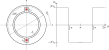
\includegraphics[width=0.8\textwidth]{fig/lec05/MMF_single_phase.pdf}
            \caption{MMF of a single-phase coil with $N$ turns for some current $i_\mathrm{a} \neq 0$ with the rotating integration path $\partial S$  along the circumference coordinate $\vartheta$. The rotor is considered an unspecific solid dummy with very high magnetic permeability.}
            \label{fig: MMF_single_phase}
    \end{figure}
\end{frame}

%%%%%%%%%%%%%%%%%%%%%%%%%%%%%%%%%%%%%%%%%%%%%%%%%%%%%%%%%%%%%
%% MMF distribution of a single-phase coil %%
%%%%%%%%%%%%%%%%%%%%%%%%%%%%%%%%%%%%%%%%%%%%%%%%%%%%%%%%%%%%%
\begin{frame}
	\frametitle{MMF distribution of a single-phase coil (cont.)}
			Utilizing Amp\`ere's law in the magnetic network context from \eqref{eq:ampere_law_magnetic_network}
            $$ \oint_{\partial S} \bm{H} \cdot \mathrm{d}\bm{s} = i_{\mathrm{f}} = N i = \sum_k  \theta_k = \sum_k l_k H_k $$
            and assuming that the air gap path along $\delta$ is dominating the magnetic circuit, we have
            \begin{equation}
                H_\mathrm{a}(\vartheta) = \frac{1}{2\delta} \theta_\mathrm{a}(\vartheta) = \frac{1}{2\delta} \begin{cases}
                    N i_\mathrm{a} & \text{for } -\pi/2 \leq \vartheta < \pi/2, \\
                    -N i_\mathrm{a} & \text{for } \pi/2 \leq \vartheta < 3\pi/2.
                \end{cases}
            \end{equation}
            \begin{figure}
                \centering
                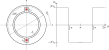
\includegraphics[width=0.5\textwidth]{fig/lec05/MMF_single_phase.pdf}
            \end{figure}
\end{frame}

%%%%%%%%%%%%%%%%%%%%%%%%%%%%%%%%%%%%%%%%%%%%%%%%%%%%%%%%%%%%%
%% Air gap flux density distribution of a single-phase coil %%
%%%%%%%%%%%%%%%%%%%%%%%%%%%%%%%%%%%%%%%%%%%%%%%%%%%%%%%%%%%%%
\begin{frame}
	\frametitle{Air gap flux density distribution of a single-phase coil}
    With $B=\mu_0 H$ in the air gap and an alternating current $i_\mathrm{a} = i_\mathrm{a}(t)$, we have
    \begin{equation}
        B_\mathrm{a}(\vartheta, t) = \frac{\mu_0}{2\delta} \begin{cases}
            N i_\mathrm{a}(t) & \text{for } -\pi/2 \leq \vartheta < \pi/2, \\
            -N i_\mathrm{a}(t) & \text{for } \pi/2 \leq \vartheta < 3\pi/2.
        \end{cases}
    \end{equation}
    \begin{figure}
        \begin{columns}
            \begin{column}{0.7\textwidth}
                \centering
		\begin{subfigure}[b]{0.45\textwidth}
			\centering
			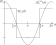
\includegraphics[width=\textwidth]{fig/lec05/B_single_phase_full_current.pdf}
			\caption{$i_\mathrm{a}(t) = \hat{i}$}
		\end{subfigure}
		\hfill
		\begin{subfigure}[b]{0.45\textwidth}
			\centering
			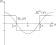
\includegraphics[width=\textwidth]{fig/lec05/B_single_phase_half_current.pdf}
			\caption{$i_\mathrm{a}(t) = \hat{i}/2$}
		\end{subfigure}
            \end{column}
            \begin{column}{0.3\textwidth}
                \caption{\raggedright Air gap flux density distribution of a single-phase coil representing a spatiotemperal function together with its fundamental component $B^{(1)}$} 
        \label{fig:Air_gap_flux_density_single_phase_coil}
            \end{column}
        \end{columns}
	\end{figure}
\end{frame}

%%%%%%%%%%%%%%%%%%%%%%%%%%%%%%%%%%%%%%%%%%%%%%%%%%%%%%%%%%%%%
%% Fourier analysis of the air gap flux density distribution %%
%%%%%%%%%%%%%%%%%%%%%%%%%%%%%%%%%%%%%%%%%%%%%%%%%%%%%%%%%%%%%
\begin{frame}
	\frametitle{Fourier analysis of the air gap flux density distribution}
        Assuming a sinusoidal current $i_\mathrm{a}(t) = \hat{i} \cos(\omega t)$, we have
        \begin{equation}
            B_\mathrm{a}(\vartheta, t) = \underbrace{\frac{\mu_0 N \hat{i}}{2\delta}}_{\hat{B}} \begin{cases}
                \cos(\omega t) & \text{for } -\pi/2 \leq \vartheta < \pi/2, \\
                -\cos(\omega t) & \text{for } \pi/2 \leq \vartheta < 3\pi/2.
            \end{cases}
            \label{eq:B_single_phase_coil}
        \end{equation}
        The flux density distribution therefore is periodic and has a sinusoidal shape over $t$ as well as a rectangular shape over $\vartheta$. To anaylze the latter in terms of its fundamental and harmonic components, we utilize the Fourier series expansion for some arbitrary $t$:
        \begin{equation}
            B_\mathrm{a}(\vartheta, t) =B_\mathrm{a}(\vartheta) = \hat{B}^{(0)} + \sum_{k=1}^{\infty} \hat{B}_{\mathrm{c}}^{(k)} \cos(k \vartheta) + \hat{B}_{\mathrm{s}}^{(k)} \sin(k \vartheta),
            \label{eq:fourier_series_B_single_phase_coil}
        \end{equation} 
        for harmonic order $k=1,2,3,\ldots$ with amplitudes $\hat{B}_{\mathrm{c}}^{(k)}$ and $\hat{B}_{\mathrm{s}}^{(k)}$. 
\end{frame}

%%%%%%%%%%%%%%%%%%%%%%%%%%%%%%%%%%%%%%%%%%%%%%%%%%%%%%%%%%%%%
%% Fourier analysis of the air gap flux density distribution (cont.) %%
%%%%%%%%%%%%%%%%%%%%%%%%%%%%%%%%%%%%%%%%%%%%%%%%%%%%%%%%%%%%%
\begin{frame}
	\frametitle{Fourier analysis of the air gap flux density distribution (cont.)}
        The coefficients of \eqref{eq:fourier_series_B_single_phase_coil} are
        \begin{equation}
            \begin{split}
                \hat{B}^{(0)} &= \frac{1}{2\pi} \int_{0}^{2\pi} B(\vartheta) \mathrm{d}\vartheta, \\
                \hat{B}_{\mathrm{c}}^{(k)} &= \frac{1}{\pi} \int_{0}^{2 \pi} B(\vartheta) \cos(k \vartheta) \mathrm{d}\vartheta, \\
                \hat{B}_{\mathrm{s}}^{(k)} &= \frac{1}{\pi} \int_{0}^{2\pi} B(\vartheta) \sin(k \vartheta) \mathrm{d}\vartheta.
            \end{split}
        \end{equation}
        For an ideal symmetrical motor and a 180$^\circ$ shifted winding configuration as in \figref{fig: MMF_single_phase}, the magnetic field does not have any offset component:
        $$\hat{B}^{(0)} = 0.$$ Furthermore, \eqref{eq:B_single_phase_coil} is an even function, i.e., $B(\vartheta)=B(-\vartheta)$ (i.e., the function is mirror-symmetrical to the $\vartheta$ axis -- cf. \figref{fig:Air_gap_flux_density_single_phase_coil}), leading to $$\hat{B}_{\mathrm{s}}^{(k)} = 0.$$
\end{frame}

%%%%%%%%%%%%%%%%%%%%%%%%%%%%%%%%%%%%%%%%%%%%%%%%%%%%%%%%%%%%%
%% Fourier analysis of the air gap flux density distribution (cont.) %%
%%%%%%%%%%%%%%%%%%%%%%%%%%%%%%%%%%%%%%%%%%%%%%%%%%%%%%%%%%%%%
\begin{frame}
	\frametitle{Fourier analysis of the air gap flux density distribution (cont.)}
        Finally, \eqref{eq:B_single_phase_coil} is symmetrical w.r.t. the abscissa, i.e., $B(\vartheta)=-B(\vartheta+\pi)$ (mirrored positive and negative half-wave), leading to
        $$\hat{B}_{\mathrm{c}}^{(k)} = 0 \quad \mbox{for } \quad k=2,4,6,\ldots .$$
        Summarizing the above, the Fourier series for the air gap flux density boils down to
        \begin{equation}
            B_\mathrm{a}(\vartheta) = \sum_{k=1,3,5,\ldots}^{\infty} \hat{B}_{\mathrm{c}}^{(k)} \cos(k \vartheta) \quad \mbox{with} \quad \hat{B}_{\mathrm{c}}^{(k)} = \frac{1}{\pi} \int_{0}^{2 \pi} B(\vartheta) \cos(k \vartheta) \mathrm{d}\vartheta.
            \label{eq:fourier_series_B_single_phase_coil_reduced}
        \end{equation}
        Utilizing symmetry of the flux distribution as shown in \figref{fig:Air_gap_flux_density_single_phase_coil}, we can calculate $\hat{B}_{\mathrm{c}}^{(k)}$ for the remaining odd $k=1,3,5,\ldots$ harmonic orders as follows:
        \begin{equation}
            \begin{split}
                \hat{B}_{\mathrm{c}}^{(k)} &= \frac{2}{\pi} \int_{-\pi/2}^{\pi/2} B(\vartheta) \cos(k \vartheta) \mathrm{d}\vartheta = \frac{\mu_0 N \hat{i}}{\delta \pi } \cos(\omega t) \int_{-\pi/2}^{\pi/2} \cos(k \vartheta) \mathrm{d}\vartheta \\ &= \frac{\mu_0 N \hat{i}}{k \delta \pi } \cos(\omega t) \left[ \sin(\frac{k \pi}{2}) - \sin(-\frac{k \pi}{2}) \right] = \frac{2 \mu_0 N \hat{i}}{\delta \pi k} \cos(\omega t) \sin(\frac{k \pi}{2}).
            \end{split}
        \end{equation}
\end{frame}

%%%%%%%%%%%%%%%%%%%%%%%%%%%%%%%%%%%%%%%%%%%%%%%%%%%%%%%%%%%%%
%% Fourier analysis of the air gap flux density distribution (cont.) %%
%%%%%%%%%%%%%%%%%%%%%%%%%%%%%%%%%%%%%%%%%%%%%%%%%%%%%%%%%%%%%
\begin{frame}
	\frametitle{Fourier analysis of the air gap flux density distribution (cont.)}
        The Fourier series describing the spatiotemperal air gap flux density distribution of a single-phase coil is therefore
    \begin{equation}
        \begin{split}
            B_\mathrm{a}(\vartheta, t) &= \frac{2 \mu_0 N \hat{i}}{\delta \pi}\cos(\omega t)\sum_{k=1,3,5,\ldots}^{\infty}   \frac{1}{k}\sin(\frac{k \pi}{2}) \cos(k \vartheta)\\ &= \frac{4}{\pi} \hat{B} \cos(\omega t)\sum_{k=1,3,5,\ldots}^{\infty}   \frac{1}{k}\sin(\frac{k \pi}{2}) \cos(k \vartheta).
        \end{split}
    \end{equation}
    One might note that $$\sin(\frac{k \pi}{2}) = 1 \quad \mbox{for } k=1,5,9,\ldots, \qquad \sin(\frac{k \pi}{2}) = -1 \quad \mbox{for } k=3,7,11,\ldots$$ applies above.  Also, the fundamental component $\hat{B}^{(1)}$ of the air gap flux density distribution is $4/\pi$ times higher than the amplitude $\hat{B}$ of the original square wave function from \eqref{eq:B_single_phase_coil} while the harmonic amplitudes decrease with $1/k$. 
\end{frame}

%%%%%%%%%%%%%%%%%%%%%%%%%%%%%%%%%%%%%%%%%%%%%%%%%%%%%%%%%%%%%
%% Fourier analysis of the air gap flux density distribution (cont.) %%
%%%%%%%%%%%%%%%%%%%%%%%%%%%%%%%%%%%%%%%%%%%%%%%%%%%%%%%%%%%%%
\begin{frame}
	\frametitle{Fourier analysis of the air gap flux density distribution (cont.)}
    \begin{columns}
        \begin{column}{0.6\textwidth}
            \begin{figure}
            \centering
            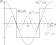
\includegraphics[width=0.825\textwidth]{fig/lec05/B_single_phase_harmonics.pdf}
            \caption{Decomposition of $B(\vartheta, t)$ for $t=0$ into its fundamental and its first harmonic components}
            \label{fig:B_single_phase_harmonics}
        \end{figure}
        \end{column}
        \begin{column}{0.4\textwidth}
            \begin{varblock}{Flux density harmonics}
                The existence of harmonics is to be attributed to the spatial distribution of the winding. The phase current was assumed to be of pure sinusoidal form, i.e., is not causing the flux density harmonics.
            \end{varblock}
        \end{column}
    \end{columns}
\end{frame}

%%%%%%%%%%%%%%%%%%%%%%%%%%%%%%%%%%%%%%%%%%%%%%%%%%%%%%%%%%%%%
%% Multipole stators %%
%%%%%%%%%%%%%%%%%%%%%%%%%%%%%%%%%%%%%%%%%%%%%%%%%%%%%%%%%%%%%
\begin{frame}
	\frametitle{Multipole stators}
        \begin{figure}
                \centering
                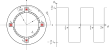
\includegraphics[width=0.8\textwidth]{fig/lec05/MMF_single_phase_two_pole_pairs.pdf}
                \caption{MMF of a single-phase coil with two pole pairs $p$ and $N/p$ turns per pole pair for some current $i_\mathrm{a} \neq 0$ with the rotating integration path $\partial S$  along the circumference coordinate $\vartheta$}
                \label{fig: MMF_single_phase_two_pole_pairs}
        \end{figure}
\end{frame}

%%%%%%%%%%%%%%%%%%%%%%%%%%%%%%%%%%%%%%%%%%%%%%%%%%%%%%%%%%%%%
%% Multipole stators (cont.) %%
%%%%%%%%%%%%%%%%%%%%%%%%%%%%%%%%%%%%%%%%%%%%%%%%%%%%%%%%%%%%%
\begin{frame}
	\frametitle{Multipole stators (cont.)}
        Following the same derivation as previously for machine with $p\geq 1$ pole pairs, we have    \begin{equation}
            \begin{split}
                B_\mathrm{a}(\vartheta, t) &= \frac{2 \mu_0 N \hat{i}}{\delta \pi p}\cos(\omega t)\sum_{k=1,3,5,\ldots}^{\infty}   \frac{1}{k}\sin(\frac{k \pi}{2}) \cos(k p \vartheta)\\ &= \frac{4}{\pi p} \hat{B} \cos(\omega t)\sum_{k=1,3,5,\ldots}^{\infty}   \frac{1}{k}\sin(\frac{k \pi}{2}) \cos(k p \vartheta).
            \end{split}
            \label{eq:B_single_phase_coil_fourier_series_multi_pole}
        \end{equation}
        Compared to the single-pole pair case, the flux density 
        \begin{itemize}
            \item amplitude is reduced by $1/p$,
            \item spatial frequency is increased by $p$: $\vartheta \rightarrow p \vartheta$. 
        \end{itemize}
        The latter implies that the fundamental and harmonics of $B(\vartheta)$ repeat $p$ times more often over the stator circumference (compare \figref{fig:B_single_phase_harmonics}).
\end{frame}

%%%%%%%%%%%%%%%%%%%%%%%%%%%%%%%%%%%%%%%%%%%%%%%%%%%%%%%%%%%%%
%% Basic rotating field model %%
%%%%%%%%%%%%%%%%%%%%%%%%%%%%%%%%%%%%%%%%%%%%%%%%%%%%%%%%%%%%%
\begin{frame}
	\frametitle{Basic rotating field model}
    \begin{columns}
		\begin{column}{0.55\textwidth}
	        We assume an ideal three-phase stator current:
            \begin{equation}
                \begin{split}
                    i_\mathrm{s,a}(t) &= \hat{i}_{\mathrm{s}} \cos(\omega t), \\
                    i_\mathrm{s,b}(t) &= \hat{i}_{\mathrm{s}} \cos(\omega t - 2\pi/3), \\
                    i_\mathrm{s,c}(t) &= \hat{i}_{\mathrm{s}} \cos(\omega t + 2\pi/3).
                \end{split}
            \end{equation}
            The index 's' indicates stator quantities, but is omitted in the following as we will only consider stator quantities until further notice, i.e.,, 
            $$i_\mathrm{s,a}(t) = i_\mathrm{a}(t), \quad i_\mathrm{s,b}(t) = i_\mathrm{b}(t), \quad i_\mathrm{s,c}(t) = i_\mathrm{c}(t)$$
            and $\hat{i}_{\mathrm{s}}=\hat{i}$. 
        \end{column}
        \begin{column}{0.45\textwidth}
            \begin{figure}
                \centering
                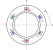
\includegraphics[width=0.8\textwidth]{fig/lec05/Simple_three_phase_stator_lumped_coils.pdf}
                \caption{Elementary three-phase stator winding with lumped coils  displaced by $120^\circ$ ($p=1$ pole pair)}
                \label{fig:Simple_three_phase_stator_lumped_coils}
            \end{figure}
        \end{column}
    \end{columns}
\end{frame}

%%%%%%%%%%%%%%%%%%%%%%%%%%%%%%%%%%%%%%%%%%%%%%%%%%%%%%%%%%%%%
%% Basic rotating field model (cont.) %%
%%%%%%%%%%%%%%%%%%%%%%%%%%%%%%%%%%%%%%%%%%%%%%%%%%%%%%%%%%%%%
\begin{frame}
	\frametitle{Basic rotating field model (cont.)}
    Transferring the finding \eqref{eq:B_single_phase_coil_fourier_series_multi_pole} to the three-phase stator winding from \figref{fig:Simple_three_phase_stator_lumped_coils} (considering an arbitrary number of $p \geq 1$ pole pairs), we have
    \begin{equation}
        \begin{split}
            B_\mathrm{a}(\vartheta, t) &= \frac{4}{\pi p} \hat{B} \cos(\omega t)\sum_{k=1,3,5,\ldots}^{\infty}   \frac{1}{k}\sin\left(\frac{k \pi}{2}\right) \cos(k p \vartheta),\\
            B_\mathrm{b}(\vartheta, t) &= \frac{4}{\pi p} \hat{B} \cos\left(\omega t - \frac{2\pi}{3}\right)\sum_{k=1,3,5,\ldots}^{\infty}   \frac{1}{k}\left(\frac{k \pi}{2}\right) \cos\left(k p \vartheta - k\frac{2\pi}{3} \right),\\ 
            B_\mathrm{c}(\vartheta, t) &= \frac{4}{\pi p} \hat{B} \cos\left(\omega t + \frac{2\pi}{3}\right)\sum_{k=1,3,5,\ldots}^{\infty}   \frac{1}{k}\left(\frac{k \pi}{2}\right) \cos\left(k p \vartheta +  k \frac{2\pi}{3}\right).
        \end{split}
        \label{eq:B_three_phase_stator_coil_fourier_series}
    \end{equation}
\end{frame}

%%%%%%%%%%%%%%%%%%%%%%%%%%%%%%%%%%%%%%%%%%%%%%%%%%%%%%%%%%%%%
%% Basic rotating field model (cont.) %%
%%%%%%%%%%%%%%%%%%%%%%%%%%%%%%%%%%%%%%%%%%%%%%%%%%%%%%%%%%%%%
\begin{frame}
	\frametitle{Basic rotating field model (cont.)}
    Applying the decomposition $$\cos(x)\cos(y) = \frac{1}{2} \left[ \cos(x-y) + \cos(x+y) \right]$$ to \eqref{eq:B_three_phase_stator_coil_fourier_series}, we obtain
    \begin{equation*}
        \small
        \begin{split}
            B_\mathrm{a}(\vartheta, t) &= \frac{2}{\pi p} \hat{B} \sum_{k=1,3,5,\ldots}^{\infty}   \frac{1}{k}\sin\left(\frac{k \pi}{2}\right)\left[\cos(\omega t - k p \vartheta) + \cos(\omega t + k p \vartheta)\right]\\
            B_\mathrm{b}(\vartheta, t) &= \frac{2}{\pi p} \hat{B} \sum_{k=1,3,5,\ldots}^{\infty}   \frac{1}{k}\sin\left(\frac{k \pi}{2}\right)\left[\cos(\omega t - k p \vartheta - \frac{2\pi}{3}(1-k)) + \cos(\omega t + k p \vartheta - \frac{2\pi}{3}(1+k))\right]\\
            B_\mathrm{c}(\vartheta, t) &= \frac{2}{\pi p} \hat{B} \sum_{k=1,3,5,\ldots}^{\infty}   \frac{1}{k}\sin\left(\frac{k \pi}{2}\right)\left[\cos(\omega t - k p \vartheta + \frac{2\pi}{3}(1-k)) + \cos(\omega t + k p \vartheta + \frac{2\pi}{3}(1+k))\right].
        \end{split}
    \end{equation*}

\end{frame}

%%%%%%%%%%%%%%%%%%%%%%%%%%%%%%%%%%%%%%%%%%%%%%%%%%%%%%%%%%%%%
%% Positive and negative sequence decomposition %%
%%%%%%%%%%%%%%%%%%%%%%%%%%%%%%%%%%%%%%%%%%%%%%%%%%%%%%%%%%%%%
\begin{frame}
	\frametitle{Positive and negative sequence decomposition}
    Hence, the decomposition led to two sinusoidal fields rotating in opposite directions:
    $$\underbrace{\cos(\omega t - k p \vartheta)=\cos(k p \vartheta - \omega t)}_{\mbox{positive sequence}} \qquad  \mbox{and} \qquad \underbrace{\cos(\omega t + k p \vartheta)}_{\mbox{negative sequence}}.$$
    \begin{figure}
        \centering
        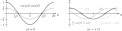
\includegraphics[width=0.9\textwidth]{fig/lec05/Positive_negative_sequence_components.pdf}
        \caption{Decomposition of the alternating field into positive and negative sequence components for $p=1$ and $k=1$}
        \label{fig:Positive_negative_sequence_components}
    \end{figure}
\end{frame}

%%%%%%%%%%%%%%%%%%%%%%%%%%%%%%%%%%%%%%%%%%%%%%%%%%%%%%%%%%%%%
%% Resulting field: positive sequence part %%
%%%%%%%%%%%%%%%%%%%%%%%%%%%%%%%%%%%%%%%%%%%%%%%%%%%%%%%%%%%%%
\begin{frame}
	\frametitle{Resulting field: positive sequence part}
    To describe the resulting field distribution (as visualized in \figref{fig:Three_phase_coils_rotating_field_animation}) 
    \begin{equation}
        B(\vartheta, t) = B_\mathrm{a}(\vartheta, t) + B_\mathrm{b}(\vartheta, t) + B_\mathrm{c}(\vartheta, t)
    \end{equation}
    we analyze the positive and negative sequences separately. Utilizing $$\cos(x \pm y) = \cos(x)\cos(y) \mp \sin(x)\sin(y)$$ we obtain for the positive sequence:
    \begin{equation*}
        \begin{alignedat}{2}
        &\cos(\omega t - k p \vartheta) &&+ \cos(\omega t - k p \vartheta - \frac{2\pi}{3}(1-k)) + \cos(\omega t - k p \vartheta + \frac{2\pi}{3}(1-k))\\
         = \quad &\cos(\omega t - k p \vartheta) &&+ \cos(\omega t - k p \vartheta) \cos(\frac{2\pi}{3}(1-k)) + \sin(\omega t - k p \vartheta) \sin(\frac{2\pi}{3}(1-k))\\
         & &&+ \cos(\omega t - k p \vartheta) \cos(\frac{2\pi}{3}(1-k)) - \sin(\omega t - k p \vartheta)\sin(\frac{2\pi}{3}(1-k)).   
        \end{alignedat}
    \end{equation*}
    Hence, the sine terms cancel out each other.
\end{frame}


%%%%%%%%%%%%%%%%%%%%%%%%%%%%%%%%%%%%%%%%%%%%%%%%%%%%%%%%%%%%%
%% Resulting field: positive sequence part (cont.) %%
%%%%%%%%%%%%%%%%%%%%%%%%%%%%%%%%%%%%%%%%%%%%%%%%%%%%%%%%%%%%%
\begin{frame}
	\frametitle{Resulting field: positive sequence part (cont.)}
    Summarizing the above, we have
        \begin{align*}
        &\cos(\omega t - k p \vartheta)  \cos(\omega t - k p \vartheta - \frac{2\pi}{3}(1-k)) + \cos(\omega t - k p \vartheta + \frac{2\pi}{3}(1-k))\\
         = \quad &\cos(\omega t - k p \vartheta)(1+2\cos(\frac{2\pi}{3}(1-k))).
    \end{align*}
    Considering $\cos(n 2 \pi)=1$ and $\cos(4\pi/3 + n 2 \pi) = \cos(2\pi/3 + n 2 \pi)=-1/2$ for $n \in \mathbb{Z}$ we observe the following for the positive sequence
    \begin{equation}
        \cos(\omega t - k p \vartheta)(1+2\cos(\frac{2\pi}{3}(1-k))) = \begin{cases}
            3 \cos(\omega t - k p \vartheta) & \text{for } k=1,7,13,19,\ldots, \\
            0 & \text{for } k=3,5,9,11,15, 17,\ldots.
        \end{cases}
    \end{equation}
    Hence, there are multiple harmonic orders which cancel out each other, among others, any multiple of $k=3$. Moreover, the positive sequences of all three phases carries the fundamental component for $k=1$.    
\end{frame}

%%%%%%%%%%%%%%%%%%%%%%%%%%%%%%%%%%%%%%%%%%%%%%%%%%%%%%%%%%%%%
%% Resulting field: negative sequence part %%
%%%%%%%%%%%%%%%%%%%%%%%%%%%%%%%%%%%%%%%%%%%%%%%%%%%%%%%%%%%%%
\begin{frame}
	\frametitle{Resulting field: negative sequence part}
    For the negative sequence part of
    \begin{equation*}
        B(\vartheta, t) = B_\mathrm{a}(\vartheta, t) + B_\mathrm{b}(\vartheta, t) + B_\mathrm{c}(\vartheta, t)
    \end{equation*}
    we rewrite the following terms
    \begin{equation*}
        \begin{alignedat}{2}
        &\cos(\omega t + k p \vartheta) &&+ \cos(\omega t + k p \vartheta - \frac{2\pi}{3}(1+k)) + \cos(\omega t + k p \vartheta + \frac{2\pi}{3}(1+k))\\
         = \quad &\cos(\omega t + k p \vartheta) &&+ \cos(\omega t + k p \vartheta) \cos(\frac{2\pi}{3}(1+k)) + \sin(\omega t + k p \vartheta) \sin(\frac{2\pi}{3}(1+k))\\
         & &&+ \cos(\omega t + k p \vartheta) \cos(\frac{2\pi}{3}(1+k)) - \sin(\omega t + k p \vartheta)\sin(\frac{2\pi}{3}(1+k))
        \end{alignedat}
    \end{equation*}
    and find for the negative sequence
    \begin{equation}
        \cos(\omega t + k p \vartheta)(1+2\cos(\frac{2\pi}{3}(1+k))) = \begin{cases}
            3 \cos(\omega t + k p \vartheta) & \text{for } k=5,11,17,\ldots, \\
            0 & \text{for } k=1, 3, 7,9,15, \ldots.
        \end{cases}
    \end{equation}
\end{frame}

%%%%%%%%%%%%%%%%%%%%%%%%%%%%%%%%%%%%%%%%%%%%%%%%%%%%%%%%%%%%%
%% Resulting field: summary %%
%%%%%%%%%%%%%%%%%%%%%%%%%%%%%%%%%%%%%%%%%%%%%%%%%%%%%%%%%%%%%
\begin{frame}
	\frametitle{Resulting field: summary}
    Combining the positive and negative sequences, we receive
    \begin{equation}
        B(\vartheta, t) = \frac{6}{\pi p} \hat{B} \sum_{k}^{\infty} \frac{1}{k} \sin\left(\frac{k \pi}{2}\right) \begin{cases}
            \cos(\omega t - k p \vartheta) & \text{for } k=1,7,13,19,\ldots, \\
            \cos(\omega t + k p \vartheta) & \text{for } k=5,11,17,\ldots, \\
            0 & \text{otherwise}.
        \end{cases}
    \end{equation}
    Utilizing $\cos(-x)=\cos(x)$ and $\sin(-x)=-\sin(x)$, we can rewrite the above as
    \begin{equation}
        B(\vartheta, t) = \frac{6}{\pi p} \hat{B} \sum_{k}^{\infty} \frac{1}{k} \sin\left(\frac{k \pi}{2}\right) \cos(\omega t - k p \vartheta) \quad \mbox{for } k=1,-5,7,-11,13,-17,\ldots.
        \label{eq:B_three_phase_stator_coil_fourier_series_resulting_field}
    \end{equation}
    Here, the negative sequences are represented by the negative harmonic orders. Finally, one can note that the amplitudes of the resulting field from the three-phase excitation \eqref{eq:B_three_phase_stator_coil_fourier_series_resulting_field} are $3/2$ times higher than in the single phase case from \eqref{eq:B_single_phase_coil_fourier_series_multi_pole}.
\end{frame}

%%%%%%%%%%%%%%%%%%%%%%%%%%%%%%%%%%%%%%%%%%%%%%%%%%%%%%%%%%%%%
%% Stator winding examples %%
%%%%%%%%%%%%%%%%%%%%%%%%%%%%%%%%%%%%%%%%%%%%%%%%%%%%%%%%%%%%%
\begin{frame}
	\frametitle{Stator winding examples}
    \begin{figure}
		\centering
		\begin{subfigure}[b]{0.49\textwidth}
			\centering
			\includegraphics[width=0.9\textwidth]{fig/lec05/Squirrel_motor_winding.jpg}
			\caption{Induction machine with fed-in stator winding  (source: \href{https://commons.wikimedia.org/wiki/File:Kommutator_eines_Universalmotor.JPGg}{Wikimedia Commons}, J. Pharos, \href{https://creativecommons.org/licenses/by-sa/3.0/deed.en}{CC~BY-SA~3.0})}
		\end{subfigure}
		\hfill
		\begin{subfigure}[b]{0.49\textwidth}
			\centering
			\includegraphics[width=0.9\textwidth]{fig/lec05/Stator_winding_at_WPS.jpg}
			\caption{Hydrogenerator with form-found stator winding (source: \href{https://commons.wikimedia.org/wiki/File:Stator_winding_at_WPS.JPG}{Wikimedia Commons},  	Astronomyinertia, \href{https://creativecommons.org/licenses/by-sa/3.0/deed.en}{CC~BY-SA~3.0})}
		\end{subfigure}
		\caption{Examples of three-phase stator windings with different configurations} 
        \label{fig:Stator_windings_examples}
	\end{figure}
\end{frame}

%%%%%%%%%%%%%%%%%%%%%%%%%%%%%%%%%%%%%%%%%%%%%%%%%%%%%%%%%%%%%
%% Winding as a distributed coil system %%
%%%%%%%%%%%%%%%%%%%%%%%%%%%%%%%%%%%%%%%%%%%%%%%%%%%%%%%%%%%%%
\begin{frame}
	\frametitle{Winding as a distributed coil system}
    In contrast to the lumped coil representation from \figref{fig:Simple_three_phase_stator_lumped_coils} the stator coils per phase are distributed over the stator circumference. To describe the winding layout, we (re-)introduce:
    \begin{gather*}
		Q: \mbox{number of slots}, \quad m: \mbox{number of phases (usually $m=3$)}, \\ q=\frac{Q}{2 p m}: \mbox{number of notches  (number of slots per phase and pole)}, \quad \rho_\mathrm{p} = \frac{\pi}{p}: \mbox{pole pitch.}
	\end{gather*}
    \begin{figure}
        \centering
        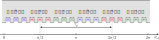
\includegraphics[width=0.8\textwidth]{fig/lec05/Scheme_distributed_winding.pdf}
        \caption{Example scheme of a distributed winding with $Q=18, p = 1, q=3$ (adapted from J.~B\"ocker, \textit{Controlled Three-Phase Drives}, Paderborn University, 2021)}
        \label{fig:Scheme_distributed_winding}
    \end{figure}
\end{frame}

%%%%%%%%%%%%%%%%%%%%%%%%%%%%%%%%%%%%%%%%%%%%%%%%%%%%%%%%%%%%%
%% Distributed winding: same width coils %%
%%%%%%%%%%%%%%%%%%%%%%%%%%%%%%%%%%%%%%%%%%%%%%%%%%%%%%%%%%%%%
\begin{frame}
	\frametitle{Distributed winding: same width coils}
    \begin{figure}
		\centering
		\begin{subfigure}[b]{0.49\textwidth}
			\centering
			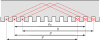
\includegraphics[height=0.35\textheight]{fig/lec05/Distributed_winding_same_width_01.pdf}
			\caption{Simplified unwound cross-section view (adapted from J.~B\"ocker, \textit{Controlled Three-Phase Drives}, Paderborn University, 2021)}
		\end{subfigure}
		\hfill
		\begin{subfigure}[b]{0.49\textwidth}
			\centering
			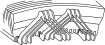
\includegraphics[height=0.35\textheight]{fig/lec05/Distributed_winding_same_width_02.pdf}
			\caption{Front view on end winding  (adapted from W.~Novender, \textit{Elektrische Maschinen}, Technische Hochschule Mittelhessen, 2023)}
		\end{subfigure}
		\caption{Realization of a distributed winding through windings of same width $y$} 
        \label{fig:Distributed_winding_same_width}
	\end{figure}
\end{frame}

%%%%%%%%%%%%%%%%%%%%%%%%%%%%%%%%%%%%%%%%%%%%%%%%%%%%%%%%%%%%%
%% Distributed winding: varying width coils %%
%%%%%%%%%%%%%%%%%%%%%%%%%%%%%%%%%%%%%%%%%%%%%%%%%%%%%%%%%%%%%
\begin{frame}
	\frametitle{Distributed winding: varying width coils}
    \begin{figure}
		\centering
		\begin{subfigure}[b]{0.49\textwidth}
			\centering
			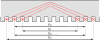
\includegraphics[height=0.35\textheight]{fig/lec05/Distributed_winding_different_width_01.pdf}
			\caption{Simplified unwound cross-section view (adapted from J.~B\"ocker, \textit{Controlled Three-Phase Drives}, Paderborn University, 2021)}
		\end{subfigure}
		\hfill
		\begin{subfigure}[b]{0.49\textwidth}
			\centering
			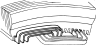
\includegraphics[height=0.35\textheight]{fig/lec05/Distributed_winding_different_width_02.pdf}
			\caption{Front view on end winding  (adapted from W.~Novender, \textit{Elektrische Maschinen}, Technische Hochschule Mittelhessen, 2023)}
		\end{subfigure}
		\caption{Realization of a distributed winding through windings of varying widths $y_i$} 
        \label{fig:Distributed_winding_different_width}
	\end{figure}
\end{frame}

%%%%%%%%%%%%%%%%%%%%%%%%%%%%%%%%%%%%%%%%%%%%%%%%%%%%%%%%%%%%%
%% Distribution factor %%
%%%%%%%%%%%%%%%%%%%%%%%%%%%%%%%%%%%%%%%%%%%%%%%%%%%%%%%%%%%%%
\begin{frame}
	\frametitle{Distribution factor}
    % fig analog to Fig. 5.2 with distributed winding
    
\end{frame}